\documentclass[11pt]{article}
\newif\ifreviewmode
\reviewmodefalse
\ifreviewmode
  \usepackage[review]{acl}
\else
  \usepackage{acl}
\fi
\usepackage{times}
\usepackage{latexsym}
\usepackage{booktabs}
\usepackage{amsmath}
\usepackage{amssymb}
\usepackage{microtype}
\usepackage{graphicx}
\usepackage{multirow}
\usepackage{fontspec}

\IfFontExistsTF{PingFang SC}{
  \newfontfamily\zhfont{PingFang SC}
}{
  \IfFontExistsTF{Songti SC}{
    \newfontfamily\zhfont{Songti SC}
  }{
    \newfontfamily\zhfont{Latin Modern Roman}
  }
}
\newcommand{\zh}[1]{{\zhfont #1}}
\emergencystretch=2.8em
\setlength{\parindent}{0pt}
\setlength{\parskip}{0pt}
\frenchspacing

\title{From Unstable Emotion Words to Stable Emotion Embeddings:\\Interpretable Tang Poetry Analysis Around the An Lushan Rebellion}

\author{Anonymous}

\begin{document}
\maketitle

\begin{abstract}
Emotion analysis for historical poetry often relies on discrete emotion words from large language models, but these outputs are prompt-sensitive and unstable for humanities interpretation.
We propose a reproducible sentence-level pipeline centered on \textbf{emotion embedding}: final-layer hidden vectors are used as continuous emotional-semantic representations; vectors are first clustered into 20 groups (\(k=20\), elbow criterion), then manually consolidated into an 18-label scheme, with an additional derived 7-class interpretative layer.
On the same 3,198 emotional sentences, one-word outputs show only 50.3\% A/B exact agreement (entropy 0.807/0.764), while embeddings maintain stable coverage (cluster entropy 0.989; 20/20 active clusters).
On 7,195 labeled sentences, a Char TF-IDF + OvR SVM baseline reaches 0.446 accuracy and 0.395 macro-F1, and year/poet analyses recover interpretable historical patterns (e.g., Sorrow peak 0.7024 in 762, a key turning point), supporting emotion embedding as a more robust and interpretable representation for digital-humanities analysis of Classical Chinese poetry.
\end{abstract}

\section{Introduction}

Large language models and modern NLP tools are increasingly used in digital humanities, but historical literary corpora remain challenging: language is archaic, supervision is sparse, and interpretative validity matters as much as predictive accuracy.
Classical Chinese poetry is a representative example.
Its emotional expression is concise and layered; a single line may compress personal grief, political anxiety, ethical commitment, and aesthetic restraint.

This paper studies emotion change around the An Lushan Rebellion (mid-8th century) as a concrete historical-literary NLP task.
Our goal is not only to improve classification scores, but to build a reproducible workflow where numeric findings can be traced back to sentence-level evidence and then reconnected to humanistic interpretation.

This study emphasizes three dimensions.
First, we formalize the core modeling steps and metrics.
Second, we add clearer validation for the representation claim that continuous embeddings are more robust than discrete generated emotion words.
Third, we expand interpretative analysis to reflect Tang poetic context and Chinese cultural semantics.

Our main contributions are:
\begin{itemize}
    \item A reproducible sentence-level pipeline for Tang poetry emotion analysis, from extraction and annotation to temporal and author-level aggregation.
    \item A two-stage label-construction chain: embedding-based automatic clustering (20 groups) for discovery, followed by manual consolidation into an 18-label scheme and a derived 7-class interpretative view.
    \item A representation comparison showing prompt sensitivity of single-word outputs and the stability/coverage advantages of continuous embeddings.
    \item Data-backed interpretative validation that links aggregate trends to concrete lines, poets, and historical context.
\end{itemize}

We position this work at the intersection of literary NLP and emotion analysis
\cite{bamman-etal-2014-bayesian,buechel-hahn-2017-emobank}.

\section{Related Work}

Computational literary studies have shown that NLP can quantify stylistic and thematic patterns while still supporting interpretative reading.
In literary NLP, modeling character and narrative signals at scale has demonstrated that probabilistic or discriminative methods can expose latent literary structure
\cite{bamman-etal-2014-bayesian}.

Emotion analysis has also moved from coarse polarity to richer representations, including multi-dimensional and perspective-aware annotations
\cite{buechel-hahn-2017-emobank}.
For Chinese Tang-poetry analysis, prior work includes hierarchical text classification for poetry corpora
\cite{xiao-2006-tang-classification},
classical machine-learning classification on Tang-poem categories
\cite{hu-zhu-2015-tang-topic},
and emotion-term extraction in digital-humanities settings
\cite{zhang-etal-2021-term-extraction}.
The Dalian emotion ontology lexicon remains a widely used lexical resource
\cite{dutir-2007-emotion-ontology},
while thesis-level studies also report limitations of relying on image-word cues alone
\cite{jiang-2020-yijing}.
For historical Chinese poetry, this motivates two design choices in our work:
(1) preserve fine-grained labels instead of collapsing directly to broad sentiment;
(2) explicitly separate computational representation from interpretative mapping.

For humanities-oriented NLP studies, methodological expectations extend beyond ``getting a score'': outputs should be auditable, stable under reasonable perturbations, and usable as evidence in humanities argumentation.
Our pipeline is designed around these constraints.

\section{Historical Framing, Data, and Annotation}

\subsection{Research Question and Event Window}

Given poem-level records with metadata (author, year, location), we ask:
\textit{how do sentence-level emotional distributions shift before, during, and after a major historical rupture, and how do those shifts differ by poet?}

We focus on the 754--764 window for year-wise comparison in this paper, centered on the rebellion era.
The analysis treats each poem as a sequence of sentence-level units.

\subsection{Data Pipeline and Canonical Set}

The workflow has two stages:
(1) sentence extraction and multi-label annotation;
(2) embedding construction, clustering, and year/poet aggregation.

To avoid denominator drift, all sentence totals and label statistics use one finalized annotated table as the canonical source.
For per-sentence label-count statistics, duplicate labels inside the same sentence are deduplicated while preserving first-occurrence order.

\begin{table}[t]
\centering
\small
\begin{tabular}{p{0.36\linewidth}p{0.48\linewidth}}
\toprule
Metric & Value / Note \\
\midrule
Total sentence rows & \textbf{10,122}; canonical annotated file \\
Rows with non-empty labels & \textbf{7,195}; used in supervised comparison \\
Rows without labels & \textbf{2,927}; retained for descriptive statistics \\
Label scheme & \textbf{18 labels, 0--3 per sentence}; obtained by manual consolidation of 20 initial clusters \\
Inter-annotator agreement & \textbf{0.970 / 0.796} (OA / Cohen's \(\kappa\); \(N{=}200\)) \\
Clustering setup & Elbow-selected \textbf{\(k=20\), \(N=3,198\)} embedding clusters for initial label discovery \\
\bottomrule
\end{tabular}
\caption{Main dataset and analysis statistics.}
\label{tab:main_results}
\end{table}

\subsection{Label System and Interpretative Layer}

The 18-label inventory is derived from, not independent of, the 20-cluster step.
We first run embedding-based unsupervised clustering and, using the elbow criterion, select \(k=20\) as an initial partition.
We then manually merge clusters with unclear semantic boundaries to form 18 annotation labels for supervised modeling.
In short, \(k=20\) serves exploratory discovery, while 18 labels serve downstream prediction and interpretation.
Primary modeling is performed on this finalized 18-label inventory.
For historical interpretation, we additionally map the 18 labels to 7 macro-categories (Sorrow, Disgust, Joy, Anger, Fear, Praise, Confusion).
This mapping is a derived analysis layer, not a replacement for the original annotation protocol.

\section{Method}

\subsection{From 20 Clusters to 18 Labels}

Given embedding vectors \(\mathbf{e}_i\), we first perform K-means for a range of \(k\) values and use the elbow curve of within-cluster sum of squares to choose \(k=20\) as the automatic initial partition.
These 20 clusters are then manually inspected and consolidated where semantic boundaries are not sufficiently clear, producing the 18-label scheme used in the supervised task.
Therefore, there is no one-to-one requirement between the 20 clusters and the 18 labels:
the former are exploratory units, the latter are annotation labels.

\subsection{18-Label Multi-Label Prediction}

Each sentence \(x_i\) has a multi-hot target vector \(\mathbf{y}_i \in \{0,1\}^{18}\).
The model predicts \(\hat{\mathbf{y}}_i\in[0,1]^{18}\) and is optimized with binary cross-entropy:
\begin{equation}
\mathcal{L} =
-\frac{1}{N}\sum_{i=1}^{N}\sum_{k=1}^{18}
\mathrm{BCE}(y_{ik},\hat{y}_{ik}),
\label{eq:bce}
\end{equation}
where
\(\mathrm{BCE}(y,\hat y)=y\log\hat y+(1-y)\log(1-\hat y)\).

We benchmark majority-label, TF-IDF word/char features with OvR Linear SVM, and TF-IDF char with OvR Logistic Regression.

\subsection{Mapping from 18 Labels to 7 Classes}

For interpretative and error-analysis views, we define a deterministic mapping
\(g:\mathcal{L}_{18}\rightarrow\mathcal{L}_{7}\).
Using a binary mapping matrix \(M\in\{0,1\}^{18\times 7}\), a sentence-level mapped target is:
\begin{equation}
\mathbf{y}^{(7)}_i = \mathbf{1}\left(M^\top\mathbf{y}^{(18)}_i > 0\right),
\label{eq:map}
\end{equation}
where \(\mathbf{1}(\cdot)\) is element-wise indicator.
This multi-hot mapped form is used for descriptive aggregation and interpretative statistics.

For the mapped 7-class classifier ablation (Table~\ref{tab:svm_mapped_ablation}), we use a diagnostic single-label projection:
take the first valid fine-grained label among \(\{\texttt{label1,label2,label3}\}\), then apply \(g\) to obtain one 7-class target.
This diagnostic setting does not replace the primary 18-label multi-label task.

\subsection{Embedding-Based Representation}

Our core innovation is to treat continuous hidden states as the primary semantic signal.
Given sentence \(x_i\), we apply a zero-shot prompt to obtain a one-word emotion output (auxiliary cue), while extracting the final-position hidden vector from the last transformer layer as embedding \(\mathbf{e}_i\in\mathbb{R}^d\).

For clustering we use K-means:
\begin{equation}
\min_{\{\mathcal{C}_j\}_{j=1}^{K}} \sum_{j=1}^{K} \sum_{\mathbf{e}_i\in\mathcal{C}_j}
\lVert \mathbf{e}_i-\boldsymbol{\mu}_j \rVert_2^2.
\label{eq:kmeans}
\end{equation}

To quantify distributional coverage across clusters, we report normalized entropy:
\begin{equation}
H_{\text{norm}} = -\frac{1}{\log K}\sum_{j=1}^{K} p_j\log p_j,
\label{eq:entropy}
\end{equation}
where \(p_j\) is cluster proportion.

\subsection{Agreement Metric}

Inter-annotator agreement is measured with Cohen's \(\kappa\):
\begin{equation}
\kappa = \frac{p_o-p_e}{1-p_e},
\label{eq:kappa}
\end{equation}
where \(p_o\) is observed agreement and \(p_e\) is chance agreement.

\subsection{Temporal and Author Aggregation}

For year \(t\) and category \(c\), ratio is computed as:
\begin{equation}
p_{c,t}=\frac{n_{c,t}}{\sum_{c'} n_{c',t}},
\label{eq:ratio}
\end{equation}
and first-order change as
\begin{equation}
\Delta p_{c,t}=p_{c,t}-p_{c,t-1}.
\label{eq:delta}
\end{equation}

These summaries support year-wise and poet-wise interpretation around the event window.

\section{Experimental Design}

\subsection{Experiment Roadmap and Roles}

To make the logic explicit for non-specialist readers, we organize experiments by role:
\begin{itemize}
    \item \textbf{E1 (Table~\ref{tab:baseline_main}):} verify that the original 18-label task is learnable and establish feature/model baselines.
    \item \textbf{E2 (Table~\ref{tab:repr_compare}):} test the core representation claim by contrasting one-word prompt outputs with continuous embeddings.
    \item \textbf{E3 (Table~\ref{tab:ablation}):} check data-leakage risk and justify grouped split as the main protocol.
    \item \textbf{E4 (Table~\ref{tab:svm_mapped_ablation}):} conduct a mapped 7-class diagnostic to examine feature and class-balance effects in a simplified setting.
    \item \textbf{E5 (Tables~\ref{tab:year_primary}--\ref{tab:poet_secondary}):} perform year/poet interpretation on canonical annotated counts, then validate with sentence-level cases.
\end{itemize}

\subsection{Task Settings and Data Subsets}

We use three fixed settings.
Setting A (primary supervised task): 18-label multi-label prediction on all rows with non-empty labels (\(N=7{,}195\)); these 18 labels come from manual consolidation of 20 initial clusters.
Setting B (diagnostic mapped task): single-label 7-class projection derived from the first valid fine-grained label per sentence.
Setting C (representation stability/discovery): a fixed emotional-sentence subset (\(N=3{,}198\)), shared by prompt A/B comparison and embedding-cluster profiling (\(k=20\)).

\subsection{Data Split and Evaluation}

Main supervised comparison uses group split by full poem (80/20), repeated over 3 seeds.
This reduces leakage from same-poem style and lexical overlap.
We report Micro-F1, Macro-F1, and exact-match subset accuracy for the 18-label task.
For Setting B, we report Macro-F1 and accuracy.

For representation comparison, we use two deterministic prompt templates (A/B) on the same 3,198 emotional sentences with DeepSeek-V3.2 (\(T{=}0\)).
The outputs are used only to test single-word stability; embedding analysis uses the continuous hidden-state vectors.

\begin{figure}[t]
\centering
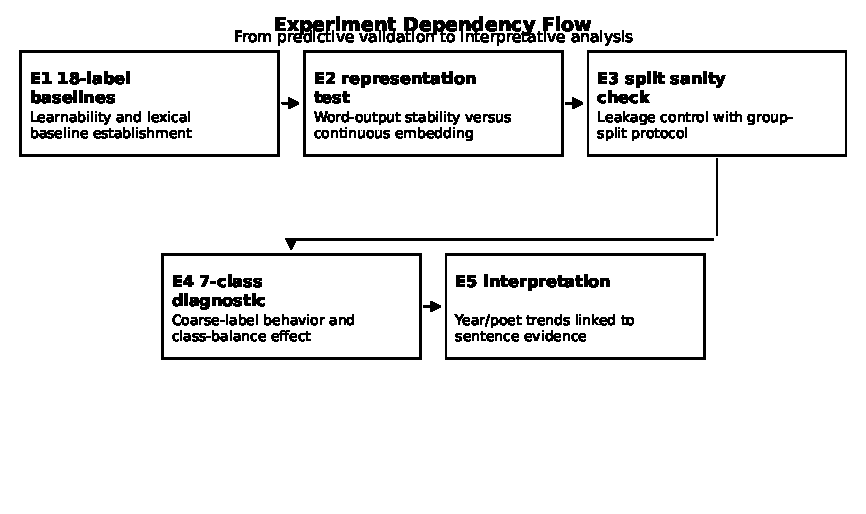
\includegraphics[width=\linewidth]{figures/experiment_dependency_flowchart.pdf}
\caption{How each experiment supports the next step in the overall argument.}
\label{fig:exp_map}
\end{figure}

Figure~\ref{fig:exp_map} summarizes the role transition from predictive validation (E1--E4) to interpretative analysis (E5).

\section{Results}

\subsection{18-Label Multi-Label Baselines}

\begin{table}[t]
\centering
\small
\resizebox{\linewidth}{!}{
\begin{tabular}{lccc}
\toprule
Model & Micro-F1 & Macro-F1 & Subset Acc. \\
\midrule
Majority-label baseline & \(0.151 \pm 0.005\) & \(0.015 \pm 0.000\) & \(0.013 \pm 0.002\) \\
Word TF-IDF (1--2) + OvR SVM & \(0.076 \pm 0.003\) & \(0.022 \pm 0.001\) & \(0.000 \pm 0.000\) \\
Char TF-IDF (1--4) + OvR SVM & \(0.446 \pm 0.003\) & \(0.395 \pm 0.007\) & \(\mathbf{0.256 \pm 0.005}\) \\
Char TF-IDF (1--3) + OvR LR & \(\mathbf{0.448 \pm 0.007}\) & \(\mathbf{0.402 \pm 0.012}\) & \(0.214 \pm 0.009\) \\
\bottomrule
\end{tabular}
}
\caption{18-label multi-label results (group split by poem, 3 seeds).}
\label{tab:baseline_main}
\end{table}

Character features substantially outperform word n-grams, consistent with Classical Chinese's weak explicit token boundaries in short lines.
SVM is best on strict subset accuracy, while LR slightly leads on Micro/Macro-F1.
Given this result, later controlled checks (Table~\ref{tab:ablation} and error analysis) use Char TF-IDF (1--4) + SVM as the anchor classifier.

\subsection{Representation Comparison: Single Word vs. Embedding}

\begin{table}[t]
\centering
\small
\resizebox{\linewidth}{!}{
\begin{tabular}{lccc}
\toprule
Setting & Consistency & Norm. H & Support \\
\midrule
Word output A & -- & \(0.807\) & 542 unique words \\
Word output B & -- & \(0.764\) & 431 unique words \\
A/B exact match & \(0.503\) & -- & 3,198 pairs \\
Embedding clustering (\(k=20\)) & N/A (continuous) & \(\mathbf{0.989}\) & \(\mathbf{20/20}\) active clusters \\
\bottomrule
\end{tabular}
}
\caption{Prompt sensitivity of single-word outputs vs. embedding coverage.}
\label{tab:repr_compare}
\end{table}

Even under deterministic decoding, A/B mismatch is \(0.497\), indicating non-trivial prompt sensitivity for discrete one-word outputs.
Embedding clusters remain fully populated (cluster size 102--257) with high normalized entropy, supporting better semantic coverage.
This experiment isolates representation stability; downstream historical trend tables are computed from canonical annotated labels rather than generated words.

\subsection{Split Sanity Check}

\begin{table}[t]
\centering
\small
\begin{tabular}{lc}
\toprule
Setting & Micro-F1 \\
\midrule
Group split by poem & \(0.446 \pm 0.003\) \\
Random sentence split & \(\mathbf{0.466 \pm 0.002}\) \\
\bottomrule
\end{tabular}
\caption{Leakage sanity check with Char TF-IDF (1--4) + OvR SVM.}
\label{tab:ablation}
\end{table}

The random split inflates performance, confirming that grouped split is the safer protocol for main reporting.

\subsection{Mapped 7-Class Single-Label Ablation}

\begin{table}[t]
\centering
\small
\resizebox{\linewidth}{!}{
\begin{tabular}{p{0.56\linewidth}cc}
\toprule
Model (7-class mapped) & Macro-F1 & Accuracy \\
\midrule
Word TF-IDF (1--3), SVM (bal.) & \(0.105 \pm 0.004\) & \(0.583 \pm 0.031\) \\
Char TF-IDF (1--3), SVM (bal.) & \(0.448 \pm 0.028\) & \(0.653 \pm 0.025\) \\
Char TF-IDF (1--4), SVM (bal.) & \(\mathbf{0.449 \pm 0.026}\) & \(0.652 \pm 0.024\) \\
Char TF-IDF (1--4), SVM (unbal.) & \(0.433 \pm 0.023\) & \(\mathbf{0.683 \pm 0.014}\) \\
\bottomrule
\end{tabular}
}
\caption{Mapped 7-class single-label diagnostic ablation.}
\label{tab:svm_mapped_ablation}
\end{table}

Balanced training improves macro fairness across rare classes, while unbalanced training favors overall accuracy.
This diagnostic result is used to understand model behavior under coarser labels, not to replace the main 18-label task.

\subsection{Temporal and Poet-Level Patterns}

All ratios in this subsection are computed from canonical annotated counts; no classifier predictions are used here.

\begin{table}[t]
\centering
\small
\resizebox{\linewidth}{!}{
\begin{tabular}{cccccccc}
\toprule
Year & Sorrow & Disgust & Joy & Anger & Fear & Praise & Confusion \\
\midrule
754 & 0.6659 & 0.0230 & 0.1590 & 0.0760 & 0.0161 & 0.0288 & 0.0311 \\
755 & 0.6269 & 0.0206 & 0.1624 & 0.1161 & 0.0154 & 0.0226 & 0.0360 \\
756 & 0.6018 & 0.0222 & 0.1519 & 0.1264 & 0.0287 & 0.0320 & 0.0369 \\
757 & 0.5664 & 0.0288 & 0.1616 & 0.1592 & 0.0168 & 0.0344 & 0.0328 \\
758 & 0.6297 & 0.0167 & 0.1862 & 0.0900 & 0.0136 & 0.0303 & 0.0335 \\
759 & 0.6463 & 0.0199 & 0.1347 & 0.1168 & 0.0223 & 0.0291 & 0.0310 \\
760 & 0.6388 & 0.0136 & 0.2097 & 0.0641 & 0.0078 & 0.0408 & 0.0252 \\
761 & 0.6276 & 0.0444 & 0.1616 & 0.0887 & 0.0158 & 0.0333 & 0.0285 \\
762 & 0.7024 & 0.0312 & 0.1239 & 0.0722 & 0.0166 & 0.0244 & 0.0293 \\
763 & 0.6653 & 0.0116 & 0.1274 & 0.1126 & 0.0189 & 0.0242 & 0.0400 \\
764 & 0.6403 & 0.0292 & 0.1278 & 0.1111 & 0.0278 & 0.0389 & 0.0250 \\
\bottomrule
\end{tabular}
}
\caption{Year-wise primary emotion ratios (754--764).}
\label{tab:year_primary}
\end{table}

\begin{table}[t]
\centering
\small
\resizebox{\linewidth}{!}{
\begin{tabular}{cccccc}
\toprule
Year & Melan. & Grief & Longing & Heroic Asp. & Romantic Aff. \\
\midrule
757 & 0.1256 & 0.1528 & 0.0696 & 0.0608 & 0.0104 \\
760 & 0.1456 & 0.0971 & 0.1029 & 0.0447 & 0.0155 \\
761 & 0.1474 & 0.1252 & 0.0856 & 0.0380 & 0.0063 \\
762 & 0.1824 & 0.1307 & 0.0985 & 0.0361 & 0.0049 \\
764 & 0.1417 & 0.1486 & 0.0750 & 0.0375 & 0.0083 \\
\bottomrule
\end{tabular}
}
\caption{Selected-year secondary emotion ratios around key turning points.}
\label{tab:year_secondary_selected}
\end{table}

\noindent\textit{Note:} Melancholy = \zh{忧伤}; Grief = \zh{悲愁}; Longing = \zh{思念};
Heroic Aspiration = \zh{壮思}; Romantic Affection = \zh{爱恋}.

\begin{table}[t]
\centering
\small
\resizebox{\linewidth}{!}{
\begin{tabular}{lccccc}
\toprule
Poet & Sent. & Melancholy & Grief & Longing & Heroic Aspiration \\
\midrule
Du Fu & 3738 & 0.1527 & 0.1709 & 0.0654 & 0.0441 \\
Li Bai & 1783 & 0.1063 & 0.1175 & 0.0595 & 0.0898 \\
Liu Changqing & 819 & 0.1783 & 0.0783 & 0.1123 & 0.0245 \\
Cen Shen & 747 & 0.1113 & 0.0799 & 0.0870 & 0.0656 \\
Dugu Ji & 276 & 0.1242 & 0.0752 & 0.1536 & 0.0523 \\
Yuan Jie & 272 & 0.0983 & 0.1838 & 0.0342 & 0.0085 \\
Gao Shi & 229 & 0.1018 & 0.1228 & 0.0632 & 0.0912 \\
Qian Qi & 200 & 0.1602 & 0.1068 & 0.1068 & 0.0534 \\
\bottomrule
\end{tabular}
}
\caption{Top-8 poets by sentence count and selected secondary emotion ratios.}
\label{tab:poet_secondary}
\end{table}

\begin{figure}[t]
\centering
\includegraphics[width=\linewidth]{../../outputs/figures/year_primary_trends.png}
\caption{Year-wise trend of three core primary emotions (Sorrow, Joy, Anger).}
\label{fig:year_primary_trend}
\end{figure}

At year level, Sorrow stays dominant and peaks in 762 (0.7024), while Joy peaks in 760 (0.2097).
Anger reaches a local peak in 757 (0.1592), then drops in 760 (0.0641).
Using Eq.~\ref{eq:delta}, notable first-order changes include \(\Delta p_{\text{Sorrow},762}=+0.0748\), \(\Delta p_{\text{Joy},760}=+0.0750\), and \(\Delta p_{\text{Anger},760}=-0.0527\).
For secondary labels, Heroic Aspiration is relatively high around 755--757 and declines in later years.
Melancholy peaks in 762, while Romantic Affection remains low throughout.

\subsection{Error Analysis and Interpretative Checks}

Using \texttt{svm\_error\_analysis\_seed42.json}, the mapped 7-class Char TF-IDF (1--4) + balanced SVM setting (Table~\ref{tab:svm_mapped_ablation}, single-seed view) yields Macro-F1 \(=0.4464\) and accuracy \(=0.6441\).
Per-class performance is uneven: Sorrow is strongest (F1 0.7732, support 879), while low-support classes remain difficult (Disgust 0.1758, support 37; Confusion 0.3871, support 29).
Top confusions include Joy\(\rightarrow\)Sorrow (86), Sorrow\(\rightarrow\)Joy (75), Sorrow\(\rightarrow\)Anger (63), and Anger\(\rightarrow\)Sorrow (55), consistent with semantically adjacent affect zones.

Interpretative counts are directly validated in the canonical table:
Heroic Aspiration in 757 appears 76 times; Melancholy in 762 appears 187 times; Romantic Affection in 762 appears 5 times.
Representative lines include \zh{时将白羽挥}, \zh{吞声不许哭}, and \zh{偏得浑家怜}.

\section{Interpretative Analysis: Tang Poetics and Cultural Context}

\subsection{Historical Shock and Emotional Restructuring}

The yearly trajectory is not a simple one-way decline; rather, the emotional structure is reorganized under accumulated historical pressure.
The Sorrow surge in 762 aligns with intensified war-aftershock memory and social dislocation in poetic expression.
To make the historical anchor explicit, our original Chinese manuscript cites \textit{Zizhi Tongjian} with the key chronology statement \citep{zizhi-tongjian-1956}:
\begin{quote}
\small
\zh{四月玄宗崩……五月肃宗崩。}
\end{quote}
In other words, Xuanzong died in the fourth lunar month and Suzong in the fifth, so major political loss and succession change were concentrated in a very short period.
This compressed historical shock provides a concrete backdrop for the emotional downturn observed in the corpus and helps explain the transition toward the more restrained tone later summarized as \zh{气骨顿衰}.
The table-level correspondence is direct.
In Table~\ref{tab:year_primary}, Sorrow peaks in 762 (0.7024), and Joy in 762 (0.1239) stays below its 760 peak (0.2097).
In Table~\ref{tab:year_secondary_selected}, Melancholy peaks in 762 (0.1824), while Romantic Affection reaches its minimum in 762 (0.0049).
Our sentence-level count check further reports Melancholy \(=187\) and Romantic Affection \(=5\) in 762.
At the same time, Joy and Anger do not vanish, suggesting that Tang poetic emotion under crisis remains multi-dimensional rather than uniformly depressive.

\subsection{Heroic Aspiration as Cultural-Ethical Signal}

Heroic Aspiration (\zh{壮思}) is most visible around 755--757 and then declines, echoing the rise and fading of what Chinese literary history calls \zh{盛唐气象}.
In Tang context, this category often overlaps with frontier rhetoric, loyalty discourse, and moral self-positioning.
Its decline in later years, together with rising Melancholy, is consistent with a shift from mobilizing rhetoric to reflective and mournful expression.

\subsection{Poet-Specific Style and Tradition}

Poet-level heterogeneity is essential for humanities interpretation.
Du Fu's high Melancholy+Grief profile supports readings of historically grounded poetic witness.
Li Bai and Gao Shi retain relatively stronger Heroic Aspiration, matching traditions of expansive voice and frontier vigor.
Thus, aggregated temporal change should be read together with poet-specific writing styles.

\subsection{Low-Frequency Affection and Genre Constraints}

Romantic Affection remains low, with a clear minimum in 762.
This does not imply absence of private emotion in Tang poetry; rather, within this wartime-centered corpus slice, public history, displacement, and political anxiety dominate the available space of expression.
The result highlights the importance of corpus framing when making cultural claims.

\section{Limitations, Ethics, and Reproducibility}

\paragraph{Interpretation boundary.}
We report structured correlations and trend alignments, not deterministic historical causality.
Computational patterns should complement, not replace, close reading.

\paragraph{Data and label limitations.}
Supervised models are trained on pipeline-generated silver labels.
A larger fully human-annotated benchmark is needed for stronger external validity and significance testing.

\paragraph{Reproducibility.}
Detailed reproducibility protocol and repository link are provided in Appendix~\ref{app:repro}.

\paragraph{Ethics.}
The study uses historical literary texts and focuses on scholarly analysis.
No personal sensitive data is involved.

\section{Conclusion}

We presented a comprehensive analysis of Tang-poetry emotion dynamics around the An Lushan Rebellion.
Methodologically, character-based baselines are strong for the 18-label task, and continuous hidden-state embeddings are more robust than single generated words for semantic analysis.
For digital humanities, the key result is that computational trends become interpretatively meaningful when they are grounded in auditable sentence-level evidence and culturally informed reading.

\appendix
\section{Reproducibility Package}
\label{app:repro}

\paragraph{Repository.}
Code, paper source, figure assets, and executable result tables are organized in:
\url{https://github.com/zhanglinyue109/anshi_emotion_analysis}.

\paragraph{Execution protocol.}
The workflow is reproduced in three stages:
(1) data preparation and annotation;
(2) supervised and representation-comparison experiments;
(3) year/poet aggregation and table generation.
All runs should log model name, prompt template version, decoding settings, random seed, and output timestamp.

\paragraph{What is packaged.}
The repository includes a dedicated package note at
\path{papers/acl_short_paper/repro_package/README.md},
which lists required scripts, expected output tables, and the minimal command order for regeneration.

\bibliography{refs}

\end{document}
